\documentclass{article}
\usepackage[utf8]{inputenc}
\usepackage{amsmath}
\usepackage{graphicx}
\usepackage[procnames]{listings}
\usepackage{color}
\usepackage{indentfirst}
\usepackage{xcolor}
\usepackage{sectsty}
\usepackage[explicit]{titlesec}
\usepackage[normalem]{ulem}
\usepackage[hidelinks]{hyperref}
\usepackage{geometry}
 \geometry{
 a4paper,
 %total={170mm,257mm},
 left=20mm,
 %top=20mm,
 }
 
 \title{\textbf{TEST RESULTS}}


\author{}
\date{}

\begin{document}

\maketitle
\begin{center}
	
\includegraphics[scale=0.6]{images/logoLIS_modified.jpg}
	\\
	\textbf{LIBRERIA}\\
	LIBRARY INFORMATION SYSTEM\\
	%\vspace{2 cm}
	Group Number : 52\\
	Group members: \\
	\begin{itemize}
		\item \begin{center}Ashrujit Ghoshal (14CS10060)\end{center}
		\item \begin{center}Sayan Ghosh (14CS10061)\end{center}
	\end{itemize}
	
\end{center}

\newpage
%\clearpage
\hypertarget{toc}{}
\tableofcontents
\newpage
\section{INTRODUCTION}
This document sketches out the test plan for Library Information Software (LIS). This prescribes the nature, purpose and methodology of all testing activities. The test plan is aimed at verifying the functionality and correct working of every aspect and part of the Library Information Software (LIS) which aims to automate the various transaction of a public library with not more than 10000 books.
\subsection{OBJECTIVE}
The software is tested using appropriate testing strategies which exhaustively test the entire program and any bugs, if detected are reported and ways to correct them are suggested.
Software Testing is an important stage in Software Development Life Cycle (SDLC).The definition of testing is the process of analyzing a software item, to detect the differences between existing and required conditions i.e. defects/errors/bugs and to evaluate the features of the software item. 
\subsection{Testing Strategy}
The strategy is to detect the differences between existing and required conditions and to evaluate the features of the software item. 

Specific test plan components include: 
\begin{enumerate}
\item Purpose for testing 
\item Items/Features to be tested
\item Pass/Fail criteria
\item Bugs if any
\end{enumerate}
 
\subsection{Scope}
The testing will be performed at several points in the life cycle as the product is constructed. Testing is a very ‘dependent’ activity. As a result, test planning is a continuing activity performed throughout the system development life cycle. Test plans must be developed for each level of product testing.
\subsection{Purpose}
The purpose of testing is to verify and validate a software to check if it fits the requirements specified and to find the bugs present in a software. The bugs found are then fixed.
 
\textbf{Bug} is a variance between the expected and actual result. The bug’s ultimate source may be traced to a fault introduced in the specification, design, or development (coding) phases. 
\section{FEATURES TO BE TESTED}
Some areas/functions in the software are to be examined and handled carefully as they are error prone. 
Majority of the users of LIS include:
Librarian
Library Clerk
Library Member

Example: \\
\begin{enumerate}
\item \textbf{Correct username, password and type combination :} If any person (Clerk/Librarian/User) try to access their accounts with unregistered usernames or with wrong passwords then the softwares raises an alert.
\item \textbf{Alert if text fields are left blank.}
\item \textbf{Unique Username:} Usernames of 2 persons cannot be same. On creating a new clerk/user with an existing username raises an alert
\item \textbf{Unique ISBN:} In case the clerk enters the ISBN number of book an existing one,then Author's name,name of book,publisher must all match,otherwise an alert is raised.
\item \textbf{Functions like issue and reserve,return are tested}. Also cases like user trying to issue/reserve a book which he has currently issued raises alert 
\item \textbf{Notifications issued to user on return of a reserved book} must be tested, as it is a complex sequential procedure.
\item \textbf{Notifications issued to librarian on overdue books},who in turn notifies the corresponding user must be tested.
\item \textbf{Statistics:}  Book issue statistics are kept for only 5 years. Issues earlier than 5 years are not reflected on the statistics.
\item \textbf{Revocation:}If an user who has reserved a book does not issue it within seven days of its return,the reservation is revoked.  And the book becomes available for issue.
\end{enumerate}

\section{Black box testing}

\begin{itemize}
	
	\item \textbf{MainWindow Login} \\
	Description : Here we test the login feature of the software once with a valid username and password combination and once with an invalid username and passowrd combination.\\
	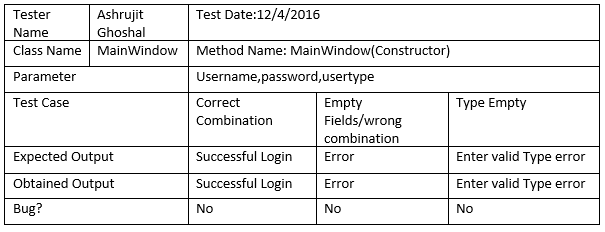
\includegraphics[scale=0.8]{images/Tables/MainWindow.PNG}\\
	
	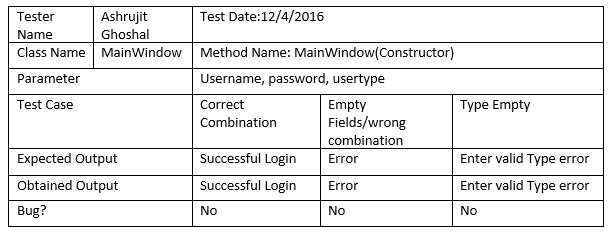
\includegraphics[scale=0.8]{images/Tables/MainWindow1.PNG}
	
	
	\item \textbf{Create user :} \\
	Description : The librarian creates the user in the system by giving the valid entries in the dialog box 'Create User'. The test has been done to see if the user can be properly created in the system. If created properly a window will be displayed confirming the creation of the new user.\\
	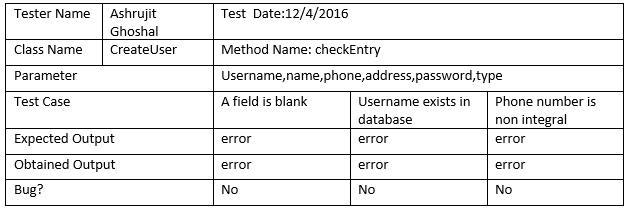
\includegraphics[scale=0.8]{images/Tables/CreateUser.PNG}
	
	\item \textbf{Create clerk :} \\
	Description : The librarian creates the clerk in the system by giving the valid entries in the dialog box 'Create Clerk'. The test has been done to see if the clerk can be properly created in the system. If created properly a window will be displayed confirming the creation of the new clerk.\\
	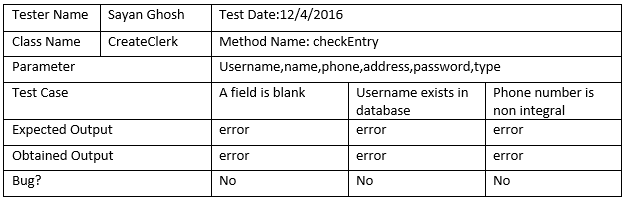
\includegraphics[scale=0.8]{images/Tables/CreateClerk.PNG}
	
	\item \textbf{Add book :} \\
	Description : The clerk adds the book in the system by giving the valid entries in the dialog box 'Add Book'. The test has been done to see if the book can be properly added in the system. If created properly a window will be displayed confirming that the book has been added to the database.\\
	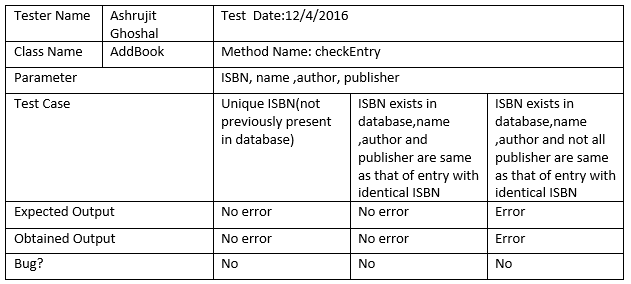
\includegraphics[scale=0.8]{images/Tables/AddBook.PNG}
	
	
	
	\item \textbf{Issue of books :} \\
	Description : Any of the valid users of the library can issue a book which is available in the library at that instant of time.\\
	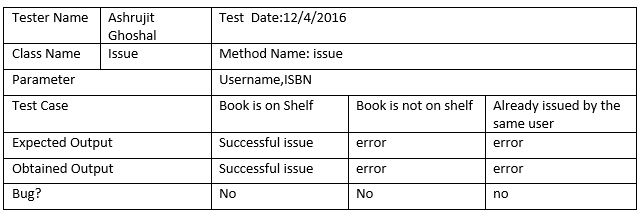
\includegraphics[scale=0.8]{images/Tables/Issue.PNG}
	
	\item \textbf{Returning books which are not reserved by anyone:} \\
	
	Description : The user who has issued the book can return the book. If the book has not been reserved by anyone beforehand then no notification is sent to the other users.\\
	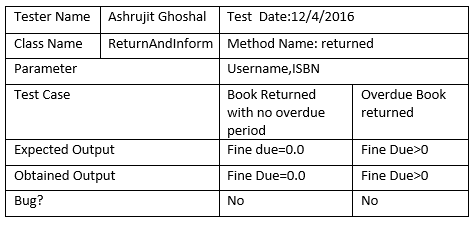
\includegraphics[scale=0.8]{images/Tables/ReturnAndInform.PNG}
	
	\item \textbf{Returning books which are reserved :} \\
	Description : The user who has issued the book can return the book and if the book has already been reserved beforehand then a notification is sent to the users who have reserved the book.\\
	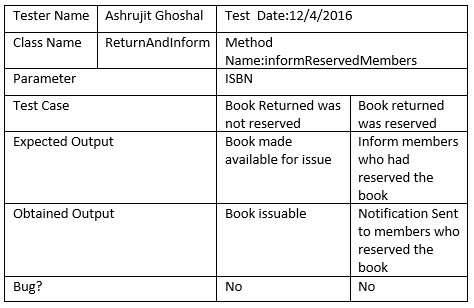
\includegraphics[scale=0.8]{images/Tables/ReturnAndInform2.PNG}
	
	\item \textbf{Reserving books :} \\
	Description : The user can reserve a book which has been issued by someone else. Whenever the book is returned the user receives a notification valid for 7 days that the said book is now available.\\
	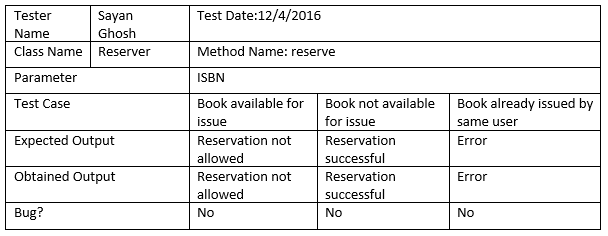
\includegraphics[scale=0.8]{images/Tables/Reserver.PNG}
	
	\item \textbf{Check Fine} \\
	Description : It is a cron job which is run by the system periodically to check if any book is overdue and if overdue case is found then the fine is calculated by the system at the rate of Re. 1 per day.\\
	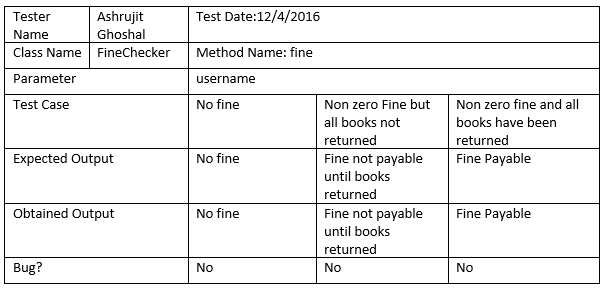
\includegraphics[scale=0.5]{images/Tables/FineChecker.PNG}
	
	\item \textbf{Remove User} \\
	Description : The librarian has the authority to delete a user from the system by using the username of the user. But the user can not be removed if he/she has any book issued against his/her account.\\
	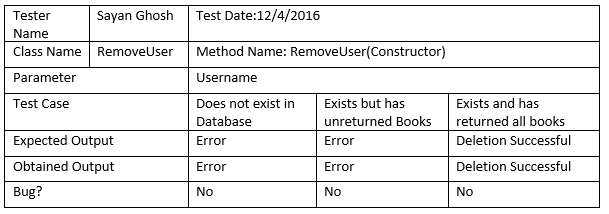
\includegraphics[scale=0.8]{images/Tables/RemoveUser.PNG}
	
	\item \textbf{Remove Clerk} \\
	Description : The librarian has the authority to remove the clerk from the system by using the username of the clerk.\\
	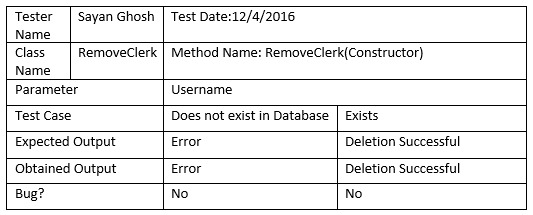
\includegraphics[scale=0.8]{images/Tables/RemoveClerk.PNG}
	
	\item \textbf{Dispose Book} \\
	Description : First the librarian issues a notification to the clerks stating that a book is to be disposed if the statistics of that book is not that good fro the last 5 years.
	Only then a valid clerk can dispose the book from the library using the ISBN code of the book.\\
	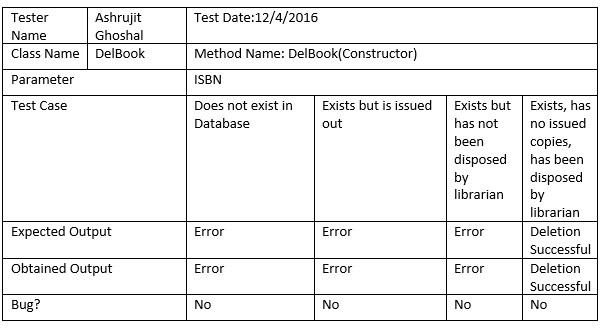
\includegraphics[scale=0.8]{images/Tables/DelBook.PNG}
	
	
	
	
\end{itemize}

\section{White box testing}
%\subsection{Integration Testing}
Librarian, Library Clerk, User are the major users/stakeholders of this software and their functions are co-dependent and inter-related. 

\begin{enumerate}
\item login into the library information system 
\begin{itemize}
\item Librarian login :\\
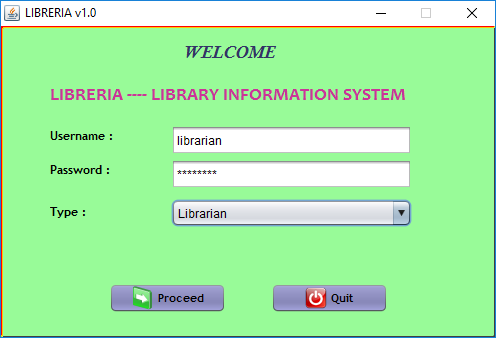
\includegraphics[scale=0.8]{images/LibrarianLogin/Login.PNG}
\\This opens up the librarian home screen as shown below:\\
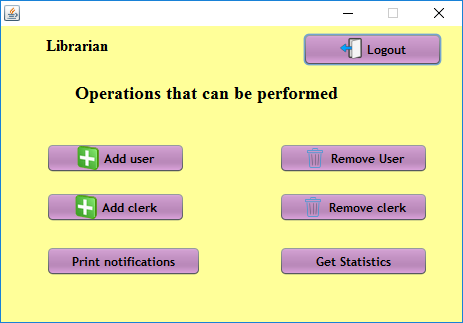
\includegraphics[scale=0.8]{images/LibrarianLogin/LibrarianHomeScreen.PNG}

\item Clerk login :\\
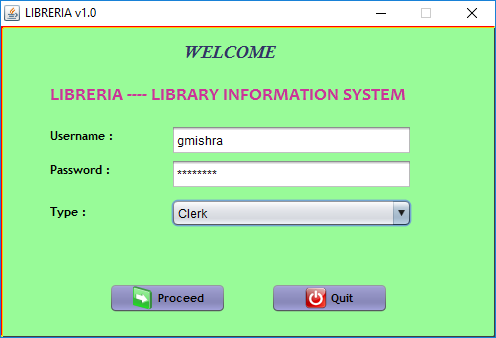
\includegraphics[scale=0.8]{images/ClerkLogin/LoginScreen.PNG}
\\This opens up the librarian home screen as shown below:\\
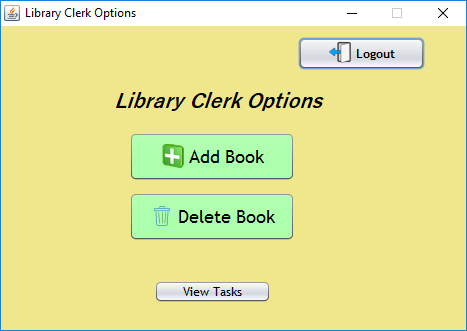
\includegraphics[scale=0.8]{images/ClerkLogin/ClerkActions.PNG}

\item User login :\\
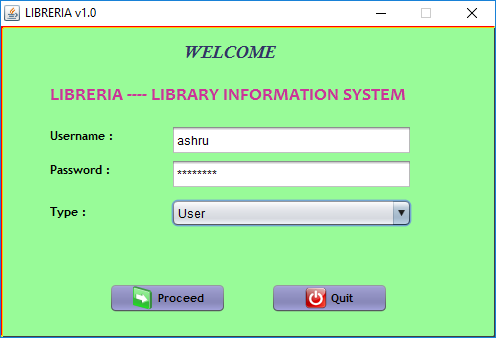
\includegraphics[scale=0.8]{images/UserLogin/LoginScreen.PNG}
\\This opens up the librarian home screen as shown below:\\
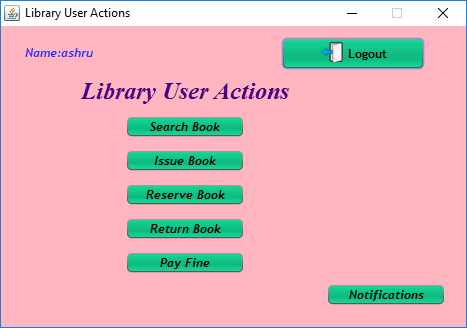
\includegraphics[scale=0.8]{images/UserLogin/UserActions.PNG}

\end{itemize}

\item Librarian creates user and clerk
\begin{itemize}
\item Creation of library user :\\
After logging in to the librarian home screen press the Add User button:\\
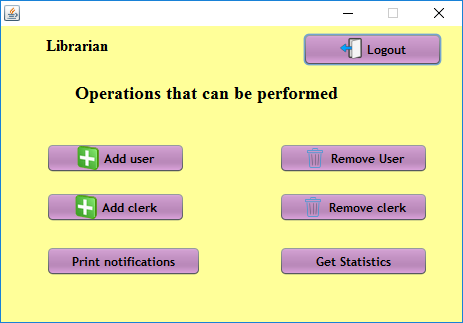
\includegraphics[scale=0.8]{images/LibrarianLogin/LibrarianHomeScreen.PNG}
%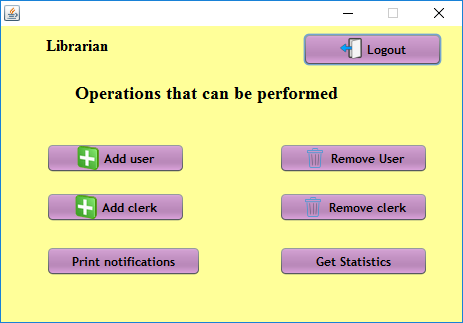
\includegraphics[scale=0.8]{images/LibrarianLogin/LibrarianHomeScreen.PNG}

\begin{itemize}
\item Creation of UG Student:\\
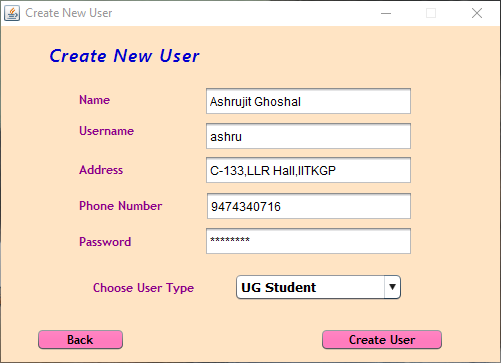
\includegraphics[scale=0.8]{images/LibrarianLogin/Actions/CreateUser/CreateUGStudent.PNG}
\item Creation of PG Student:\\
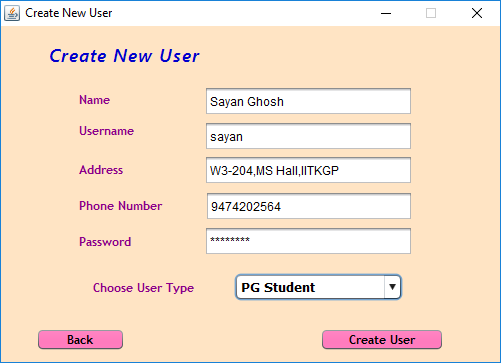
\includegraphics[scale=0.8]{images/LibrarianLogin/Actions/CreateUser/CreatePGStudent.PNG}
\item Creation of Research Scholar:\\
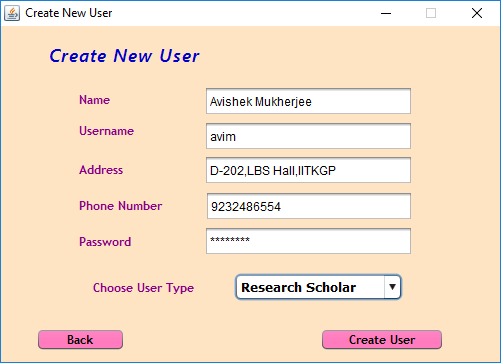
\includegraphics[scale=0.8]{images/LibrarianLogin/Actions/CreateUser/CreateResearchScholar.PNG}
\item Creation of Faculty:\\
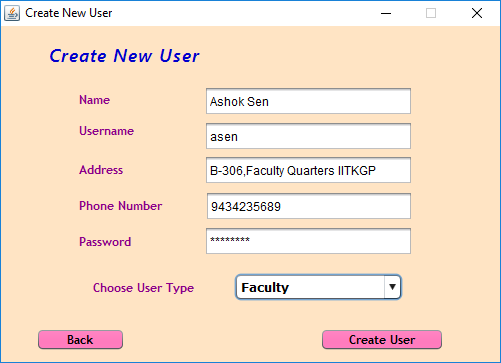
\includegraphics[scale=0.8]{images/LibrarianLogin/Actions/CreateUser/CreateFaculty.PNG}
\\
\textbf{Expected Result:}\\
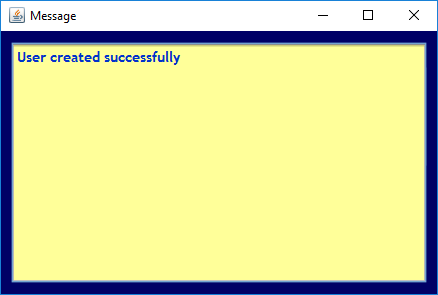
\includegraphics[scale=0.8]{images/LibrarianLogin/Actions/CreateUser/SuccessfullyCreated.PNG}
\\
\textbf{Result Obtained:}\\
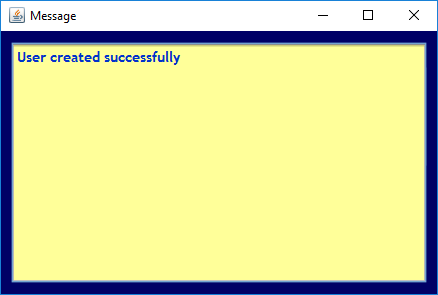
\includegraphics[scale=0.8]{images/LibrarianLogin/Actions/CreateUser/SuccessfullyCreated.PNG}
\\

\end{itemize}


\item Create Clerk :\\
After logging in to the librarian home screen press the Add Clerk button:\\
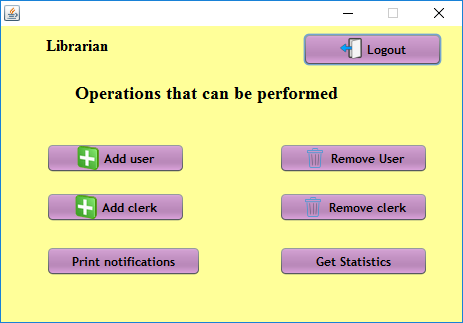
\includegraphics[scale=0.8]{images/LibrarianLogin/LibrarianHomeScreen.PNG}\\
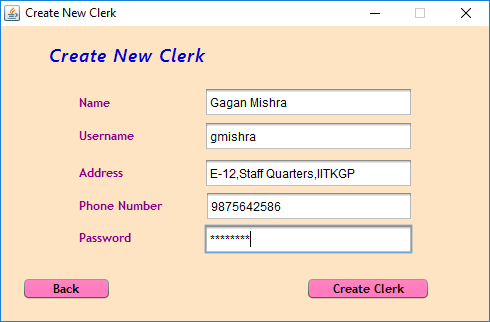
\includegraphics[scale=0.8]{images/LibrarianLogin/Actions/CreateClerk/ClerkDetails.PNG}\\\
\textbf{Result expected :}
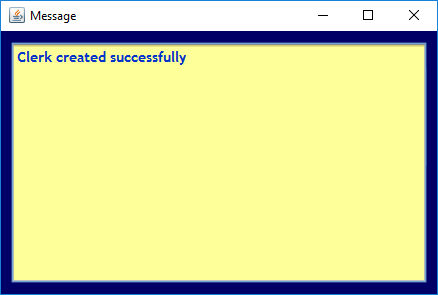
\includegraphics[scale=0.8]{images/LibrarianLogin/Actions/CreateClerk/ClerkCreated.PNG}\\
\textbf{Result Obtained :}
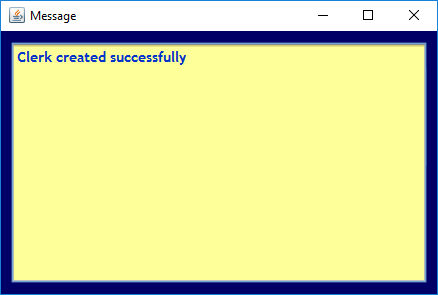
\includegraphics[scale=0.8]{images/LibrarianLogin/Actions/CreateClerk/ClerkCreated.PNG}\\


\end{itemize}
\item Library clerk adds book\\
After going to ClerkHomeScreen the clerk clicks on Add Book\\
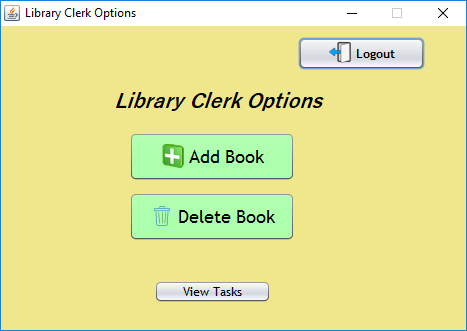
\includegraphics[scale=0.8]{images/ClerkLogin/ClerkActions.PNG}\\
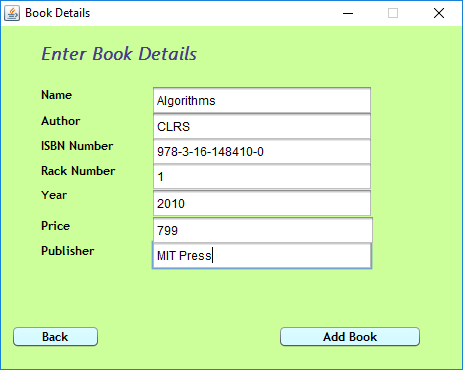
\includegraphics[scale=0.8]{images/ClerkLogin/Actions/AddBook/BookDetails.PNG}\\
Then click on Add Book button\\
\textbf{Expected Result :}\\
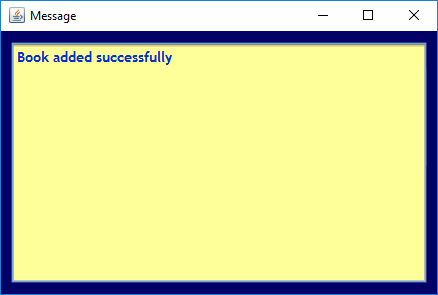
\includegraphics[scale=0.8]{images/ClerkLogin/Actions/AddBook/BookAdded.PNG}\\
\textbf{Result Obtained :}\\
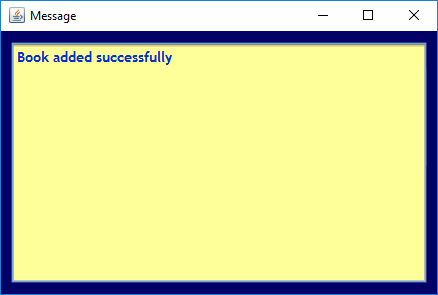
\includegraphics[scale=0.8]{images/ClerkLogin/Actions/AddBook/BookAdded.PNG}\\

\item User issues,reserves,returns,searches book and pays fine \\
First the user has to successfully login and the UserHomeScreen opens up :\\
\begin{itemize}
\item Search Book :\\
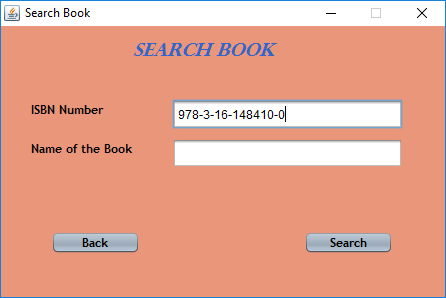
\includegraphics[scale=0.8]{images/UserLogin/Actions/SearchExisting/SearchByISBN/SearchExistingBook.PNG}\\
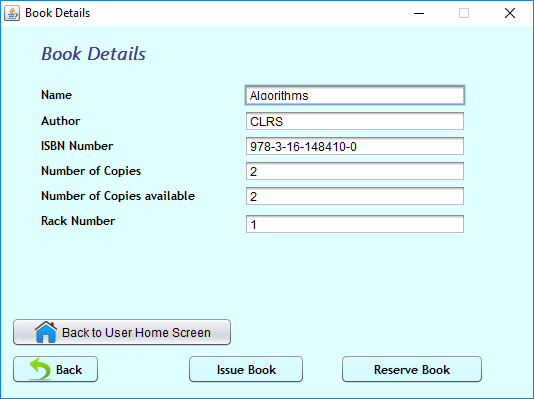
\includegraphics[scale=0.8]{images/UserLogin/Actions/SearchExisting/SearchByISBN/SearchExistingBookFound.PNG}\\

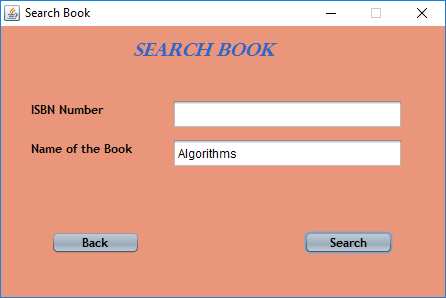
\includegraphics[scale=0.8]{images/UserLogin/Actions/SearchExisting/SearchByName/SearchExistingBook.PNG}\\
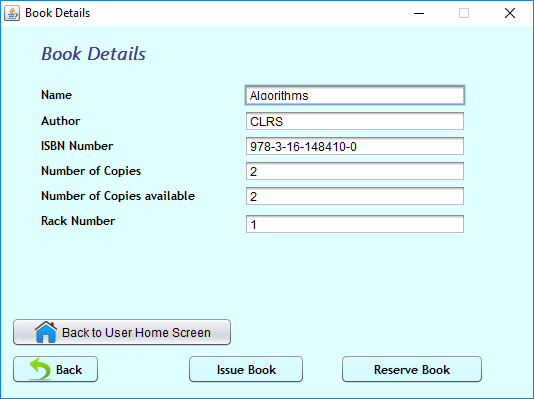
\includegraphics[scale=0.8]{images/UserLogin/Actions/SearchExisting/SearchByName/Found.PNG}\\

\item Issue Book: \\
\textbf{Path 2:}
After searching for the book in the previous step click on 'Issue Book' button :\\
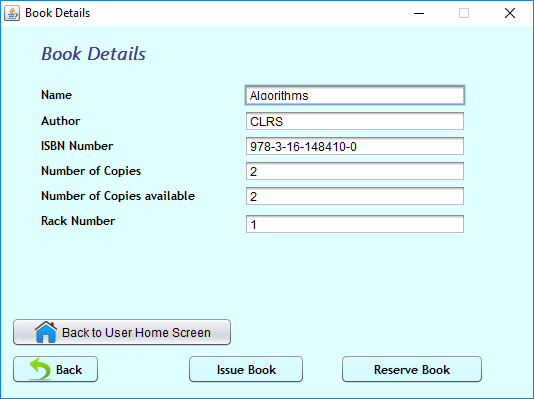
\includegraphics[scale=0.8]{images/UserLogin/Actions/SearchExisting/SearchByName/Found.PNG}\\
\textbf{Expected Result :}\\
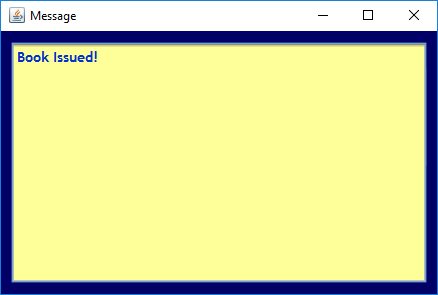
\includegraphics[scale=0.8]{images/UserLogin/Actions/BookIssued.PNG}\\
\textbf{Result Obtained :}\\
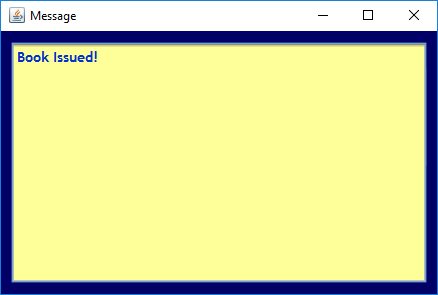
\includegraphics[scale=0.8]{images/UserLogin/Actions/BookIssued.PNG}\\

\textbf{Path 2:}
The user can also issue the book from the complete book list instead of the searching the book everytime . \\
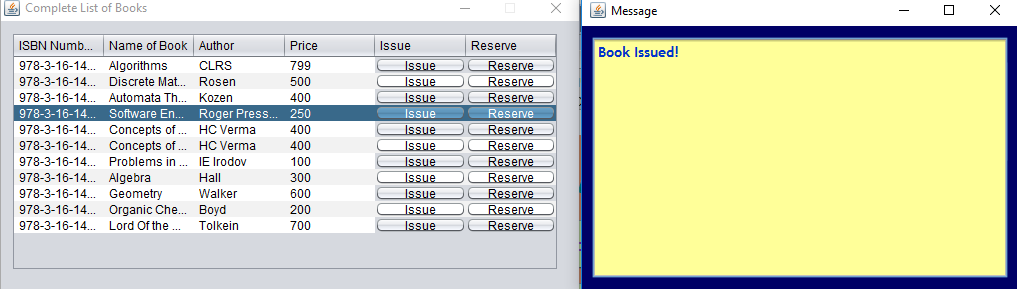
\includegraphics[scale = 0.5]{images/UserLogin/Actions/Reserve_reserveNotif/Issuefirst.PNG}\\


In case the user tries to issue the book already then he faces the following error.\\
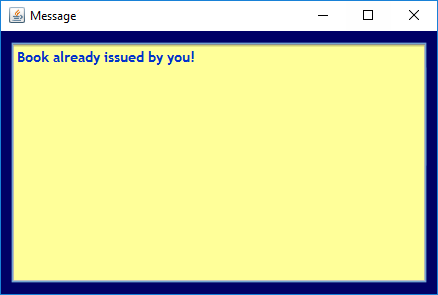
\includegraphics[scale =0.8]{images/UserLogin/Actions/IssuedAlreadyError.PNG}\\

\item Reserve Book\\
\textbf{Path 1:}
After searching for the book in the previous step click on 'Reserve Book' button :\\
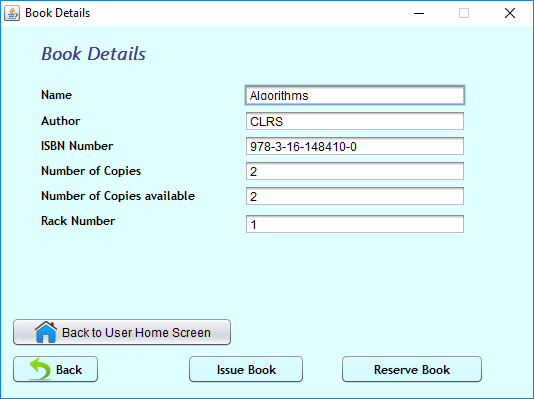
\includegraphics[scale=0.8]{images/UserLogin/Actions/SearchExisting/SearchByName/Found.PNG}\\

\textbf{Expected Result :}\\
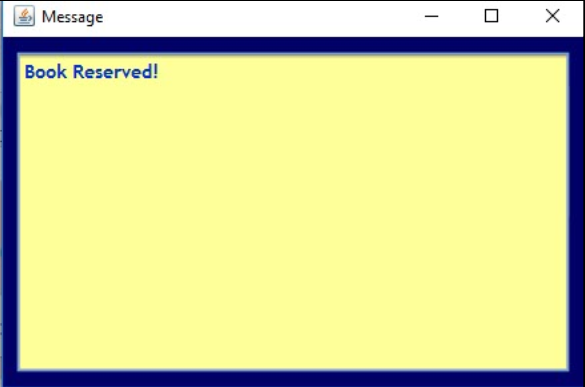
\includegraphics[scale=0.8]{images/BookReserved.PNG}\\
\textbf{Result Obtained :}\\
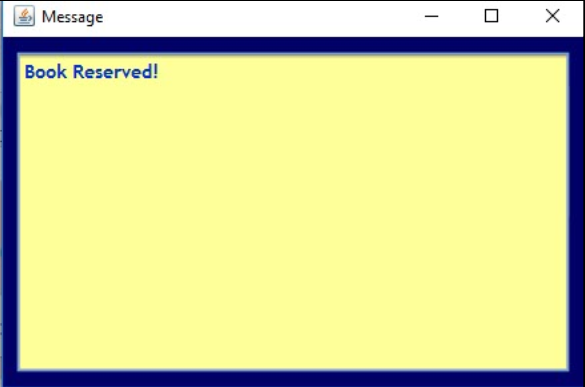
\includegraphics[scale=0.8]{images/BookReserved.PNG}\\

\textbf{Path 2:}
The user can also reserve the book from the complete book list instead of the searching the book everytime . \\
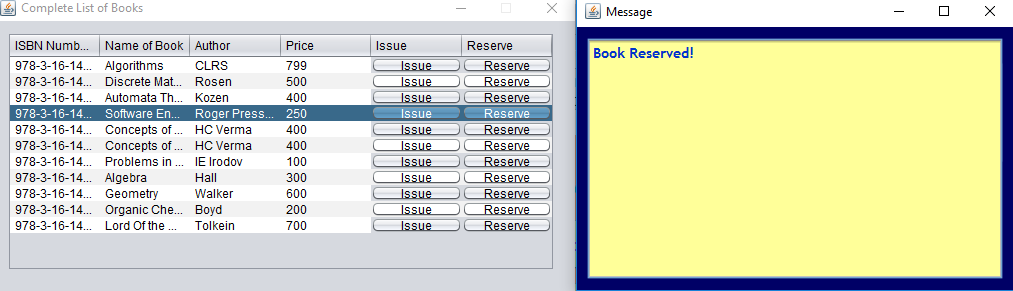
\includegraphics[scale = 0.5]{images/UserLogin/Actions/Reserve_reserveNotif/BookReserved.PNG}\\


In case the user who has issued tries to reserve the same book again the following result is displayed :\\
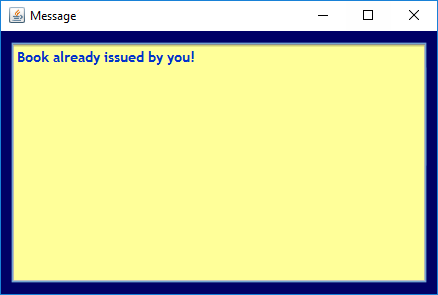
\includegraphics[scale =0.8]{images/UserLogin/Actions/IssuedAlreadyError.PNG}\\

In case the user tries to reserve a book already available the following error is displayed :\\
\includegraphics[scale =0.8]{images/UserLogin/Actions/ReserveError.PNG}\\


\item Return book :\\

After reaching the user home screen the user needs to click on the Return Book button.\\
The following window opens up showing the list of the books already issued.\\

\includegraphics[scale = 0.8]{images/UserLogin/Actions/ReturnScreen.PNG}\\
Then the user clicks on the Return button beside the specific book.\\
\includegraphics[scale = 0.8]{images/UserLogin/Actions/BookReturned.PNG}\\

If the book has been returned then a Reserve Notification is issued to those users who had reserved that book.\\
\includegraphics[scale=0.8]{images/UserLogin/UserActions.PNG}\\
\includegraphics[scale=0.8]{images/UserLogin/Actions/NotificationWindow.PNG}\\
\includegraphics[scale=0.8]{images/UserLogin/Actions/Reserve_reserveNotif/ReserveNotif.PNG}\\

Advancement of 7 days removes the notification from the book from the list.\\
\includegraphics[scale=0.8]{images/UserLogin/Actions/Reserve_reserveNotif/Reservenotifcancelledafter7days.PNG}\\


\end{itemize}
\item Librarian can delete user and clerk
\begin{itemize}
\item Remove User :\\
Librarian after successful login clicks on the 'Remove User' button\\
Now, the Remove User dialog box opens up\\
\includegraphics[scale=0.8]{images/LibrarianLogin/Actions/DeleteUser/DeleteUserScreen.PNG}\\
Now, press the 'Remove User' button,\\
\textbf{Result Expected :}\\
\includegraphics[scale=0.8]{images/LibrarianLogin/Actions/DeleteUser/UserDeleted.PNG}\\
\textbf{Result Obtained :}\\
\includegraphics[scale=0.8]{images/LibrarianLogin/Actions/DeleteUser/UserDeleted.PNG}\\

\item Remove Clerk:\\
Librarian after successful login clicks on the 'Remove Clerk' button\\
Now, the Remove Clerk dialog box opens up\\
\includegraphics[scale=0.8]{images/LibrarianLogin/Actions/DeleteClerk/DeleteScreen.PNG}\\
Now, press the 'Remove Clerk' button,\\
\textbf{Result Expected :}\\
\includegraphics[scale=0.8]{images/LibrarianLogin/Actions/DeleteClerk/ClerkDeleted.PNG}\\
\textbf{Result Obtained :}\\
\includegraphics[scale=0.8]{images/LibrarianLogin/Actions/DeleteClerk/ClerkDeleted.PNG}\\

\end{itemize}


\item Library clerk can delete a book from database after librarian  gives a notification to dispose it\\
First a librarian has to notify clerk regarding the books to dispose off, without these notification the clerk is not allowed to dispose any book.\\

\includegraphics[scale = 0.8]{images/ClerkLogin/Actions/DeleteBook/ClerkNotif.PNG}\\
\includegraphics[scale = 0.8]{images/ClerkLogin/Actions/DeleteBook/DisposeWindow.PNG}\\
\includegraphics[scale = 0.8]{images/BookDisposed.PNG}\\

\item Book Issue limit :\\
\begin{itemize}
	

	
\item Book Limit reached for UG students :\\
Showing 2 books already issued\\
\includegraphics[scale=0.8]{images/BookLimitUG.PNG}\\
Again trying to issue,\\
\textbf{Result Expected :}\\
\includegraphics[scale=0.8]{images/BookLimitError.PNG}\\
\textbf{Result Obtained :}\\
\includegraphics[scale=0.8]{images/BookLimitError.PNG}\\
\item Book Limit reached for PG students :\\
Showing 4 books already issued\\
\includegraphics[scale=0.8]{images/BookLimitPG.png}\\
Again trying to issue,\\
\textbf{Result Expected :}\\
\includegraphics[scale=0.8]{images/BookLimitError.PNG}\\
\textbf{Result Obtained :}\\
\includegraphics[scale=0.8]{images/BookLimitError.PNG}\\
\item Book Limit reached for Research Students :\\
Showing 6 books already issued\\
\includegraphics[scale=0.8]{images/BookLimitRS.PNG}\\
Again trying to issue,\\
\textbf{Result Expected :}\\
\includegraphics[scale=0.8]{images/BookLimitError.PNG}\\
\textbf{Result Obtained :}\\
\includegraphics[scale=0.8]{images/BookLimitError.PNG}\\
\item Book Limit reached for Faculty :\\
Showing 10 books already issued\\
\includegraphics[scale=0.8]{images/BookLimitFaculty.PNG}\\
Again trying to issue,\\
\textbf{Result Expected :}\\
\includegraphics[scale=0.8]{images/BookLimitError.PNG}\\
\textbf{Result Obtained :}\\
\includegraphics[scale=0.8]{images/BookLimitError.PNG}\\
\end{itemize}


	\item Pay Fine :\\
	The user has to pay fine if any of the book is overdue.\\
	In case of overdue the return book screen looks like this.\\
	\includegraphics[scale=0.8]{images/UserLogin/Actions/OverdueBookFine.PNG}\\
	
	Also the user receives a notification in the Overdue Notifications pane of the Notification section of the user when user clicks on the Notifications button and then on the Overdue Notifications Button.
	
	\includegraphics[scale=0.8]{images/UserLogin/UserActions.PNG}\\
	\includegraphics[scale=0.8]{images/UserLogin/Actions/NotificationWindow.PNG}\\
	\includegraphics[scale=0.8]{images/UserLogin/Actions/OverdueNotifications.PNG}\\
	Then after the return of the books the user can pay fine by clicking on the Pay Fine button on the home screen of the user.\\
	
	After clicking on that button the fine is paid.\\
	
	\textbf{Result Expected :}\\
	\includegraphics[scale=0.8]{images/UserLogin/Actions/PayFineSucessful.PNG}\\
	\textbf{Result Obtained :}\\
	\includegraphics[scale=0.8]{images/UserLogin/Actions/PayFineSucessful.PNG}\\
	
	
	In case there is no fine then the following result is displayed.\\
	\includegraphics[scale=0.8]{images/UserLogin/Actions/PayFineError.PNG}\\
	
	
	\item Issue Statistics:\\
	The librarian can view the statistics of the books present in the library.\\
	\includegraphics[scale=0.8]{images/LibrarianLogin/Actions/IssueStats/NormalIssueStats.PNG}\\
	Advancing date by 5 years the Issue Statistics changes as follows:\\
	\includegraphics[scale=0.8]{images/LibrarianLogin/Actions/IssueStats/IssueStatsAfter5years.PNG}	
\end{enumerate}


%\subsection{Conversion Testing}
\section{Interface Testing}
Upon clicking a button a new window pops up whenever required. Care is taken that the program doesn’t shut down abruptly if some intermediate window is closed.\\
In order to reduce the number of windows displayed on the screen care has been taken to show only one window on the screen wherever possible and the transition between the windows is fast.\\
When the user or the clerk home screen is closed he/she is automatically logged out of the system and the main window is displayed again.\\
When closing the main window a confirmation dialog box opens up asking the user to confirm if he/she wants to exit from the software.\\
\section{Security Testing}
If a person tries to access the software using invalid usernames and passwords then an alert is raised.\\
Also during the disposal of a book the clerk has to receive a notification to do the same otherwise the book will not be disposed. So in other words, the librarian has the sole authority to give an order to dispose the books, the clerk is only performing the action.\\
Now showing below the test results :\\
\begin{itemize}
\item Trying to login with wrong combination of username and password:\\
\includegraphics[scale=0.8]{images/WrongUsername.PNG}
\\\textbf{Expected result :}\\
\includegraphics[scale=0.8]{images/LoginError1.PNG}\\
\textbf{Result Obtained :}\\
\includegraphics[scale=0.8]{images/LoginError1.PNG}\\


\end{itemize}
\section{Regression Testing}
For this problem specification no regression testcases are present and hence no regression testing has been done.
\end{document}